\documentclass{eceasst}
% This is the source of the author documentation
% for the ECEASST document class.

% Required packages
% =================
\usepackage{subfig}

% Volume frontmatter
% ==================
% Volume frontmatter for OCL 2011
% =====================================
\volume{44}{2011} % Volume number and year
\volumetitle{% Title of the volume (optional)
Proceedings of the\\
Workshop on OCL and Textual Modelling\\
(OCL 2011)}
\volumeshort{% Short title of the volume (optional)
Proc.\ OCL 2011}
\guesteds{% Multiple guest editors
Jordi Cabot, Robert Clariso, Martin Gogolla, Burkhart Wolff}

% Article frontmatter
% ===================
\title{% Title of the article
Aligning OCL with UML}
%\short{% Short title of the article (optional)
%Aligning OCL with UML}
\author{% Authors and references to addresses
Edward Willink\autref{1}}
\institute{% Institutes with labels
\autlabel{1} \email{ed \_at\_ willink.me.uk}, \url{http://www.eclipse.org/modeling}\\
Eclipse Modeling Project}

\abstract{
OCL is widely used by UML and other languages to constrain meta-models and perform evaluations on models.
Unfortunately no OCL 2.x specification has ever been aligned with any UML 2.x specification. This lack of alignment makes some OCL compliance points such as XMI interchange unachievable. This paper describes how introduction of an OCL Pivot Meta-Model and clear exposition of the Values package may provide a solution to the alignment and a variety of other specification issues.}
\keywords{OCL, meta-model, pivot model, library, auto-generation, templates}

\begin{document}
\maketitle
\section{Introduction}

The Object Constraint Language (OCL) evolved, initially within the Unified Modeling Language (UML). As part of the UML 2.0\cite{UML-2.0} revision activities, OCL was separated out as a separate specification in recognition of OCL's utility in non-UML contexts. Unfortunately the UML Revision Task Force had insufficient resources to complete the revision of OCL 1.6\cite{OCL-1.6} to align with UML 2.0. A partially revised OCL 2.0 draft\cite{OCL-2.0-draft} was all that was available to accompany UML 2.0.

When the QVT specification was developed, the utility of OCL was recognized and OCL 2.0\cite{OCL-2.0} formed the basis for QVT 1.0\cite{QVT-1.0}. The QVT Finalization Task Force also finalized the OCL 2.0 specification, but  had insufficient resources to perform the very detailed proof reading and consistency checking for a specification involving so many cross-references.

Subsequent revisions \cite{OCL-2.2},\cite{OCL-2.3} have addressed a number of  inconsistencies, but the major problems remain unaddressed.

Each version of OCL 2.x states in its Scope statement that it is aligned with the corresponding UML 2.x specification. Sadly this statement is only an aspiration at present. In this paper we examine the major misalignments and outline a proposal to resolve these and other minor misalignments.

It is hoped that by presenting the community with an early insight into changes that may be proposed for OCL 2.4, the community may be able to contribute constructively before, rather than after, the revised specification is adopted.

A prototype of the UML-aligned OCL meta-models may be found in the optional Examples and Editors of the Indigo release of Eclipse OCL, which is officially released in June 2011 and for which milestone builds have been available since December 2010. The prototype uses fully automated conversion starting with potentially standard UML meta-models for OCL and UML deriving a merged OCL Pivot Meta-Model and associated Eclipse Ecore tooling. Despite the use of Ecore tooling, with this approach the name of a meta-class is an OMG-compliant `Class' rather than the Ecore `EClass'. 

The UML-alignment outlined below involves very few if any, actual changes to the concrete syntax and semantics of OCL; they merely enable the specification to say what many users think it already says. However the changes to the meta-modeling for OCL tooling is quite significant.

In Section \ref{Background} we discuss the OCL specification and the way it is used. Then in Section \ref{Problems} we  identify a number of problems for which we propose solutions in Section \ref{Solutions}. Finally we conclude. 

\section{Background}\label{Background}

Although the OCL specification is partitioned very logically, it can appear that the specification contains more information than is necessary.

\begin{itemize}
\item Clause 7 provides a non-normative and readable overview of OCL
\item Clause 8 specifies the Abstract Syntax, comprising the Types and Expressions classes that define the executable language, 
\item Clause 9 specifies the Concrete Syntax for the grammar and non-normative Concrete Syntax classes that define the readable language, 
\item Clause 10 specifies the Evaluation semantics using the Values and Evaluations classes to define the behavior, 
\item Clause 11 specifies the OCL Standard Library which provides the operations and iterations that make Types useful, 
\item Clause 12 specifies the Complete OCL language, an ability to define an independent OCL Document that complements a pre-existing meta-model.
\item Annex A provides a more formal but non-normative foundation for OCL semantics
\end{itemize}

A problem in understanding the specification, is that constraints that apply solely to the AST are found in Clause 8, constraints that affect construction of the AST are found in Clause 9, and constraints that affect execution of the AST are found in Clause 10, while the operations used in constraints are in Clause 11.

Much of Clause 10 on Evaluation seems strange, irrelevant and repetitious, but it serves an important and surprisingly practical purpose that we discuss in Section \ref{Values}.

Comparison of Clause 12 on Complete OCL with the preceding clauses quickly reveals that Clause 12 is a bit thin; Clause 12 is still a preliminary draft, and it is in realizing Clause 12 that the major UML alignment issues arise. We discuss these in Section \ref{CompleteOCL}.
 
\subsection{OCL Compliance Points}

The OCL specification defines three major compliance points, with additional minor options for evaluation.

\subsubsection{Concrete Syntax}

Interchange of concrete syntax between tools is moderately successful today, but is limited by ambiguities in the specification and consequent divergent misunderstandings by tool implementors. These difficulties should be significantly alleviated by a sound OCL Standard Library model as described in our companion paper\cite{OCL-stdlib}.
 
\subsubsection{XMI Interchange}

XMI Interchange is important to allow the costs of parsing the Concrete Syntax to be isolated from execution costs. In the XMI representation, all syntax sugar is removed and references directly access target features using properties such as OperationCallExp::referredOperation. This requires the target operation to have a URI, which is true of user models. However the OCL Standard Library has no model and policy for establishing URIs independent of a model, so XMI Compliance is impossible whenever a library operation is used.

The Eclipse MOFM2T\cite{MOFM2T} implementation (Acceleo\cite{M2T/Acceleo}) exploits XMI interchange to compile a complete Model to Text transformation on completion of an edit and so accelerate the subsequent execution of the transformation from the compiled binary program captured as an XMI model. The deficiency in the OCL specification of URIs therefore ripples to MOFM2T forcing Acceleo to adopt proprietary solutions for its compiled representation. The problems with basic URIs are addressed by a providing a model for the OCL Standard Library as described in our companion paper\cite{OCL-stdlib}.

More serious URI problems arise with underspecification of Complete OCL and we address these in Section \ref{CompleteOCL}.

\subsubsection{Evaluation semantics}

The specification requires that tools evaluate in accordance with OCL semantics, which is a relatively modest requirement for basic arithmetic values, but becomes quite troublesome for null, invalid and very large or high precision values.

The specification provides no API by which a query can be invoked and so the only way to test an OCL expression is through its contribution to the satisfaction of an invariant, or the value returned by a modeling environment that exploits OCL to realize an operation body or a property initialization or derivation. In each case the value returned by the OCL tooling is passed through the environment supporting OCL before it can be observed. It is therefore not possible to detect whether an OCL tool uses the classes specified in the Values package. Practical tools do not and this has allowed some significant problems in the Values package to remain unreported. We address these in Section \ref{Values}.
 
\subsection{OCL Usage}

A standard way of using UML is shown in Figure~\ref{fig:BasicScenario}. A UML model conforming to a UML meta-model is maintained by an editing activity. When appropriate this model is exported to an EMOF (or Ecore) model conforming to a corresponding meta-model. The EMOF model contributes to a code generation activity that produces a program that can be executed to exploit EMOF objects that are instances that instantiate classes from the EMOF model.

\begin{figure}
  \begin{center}
    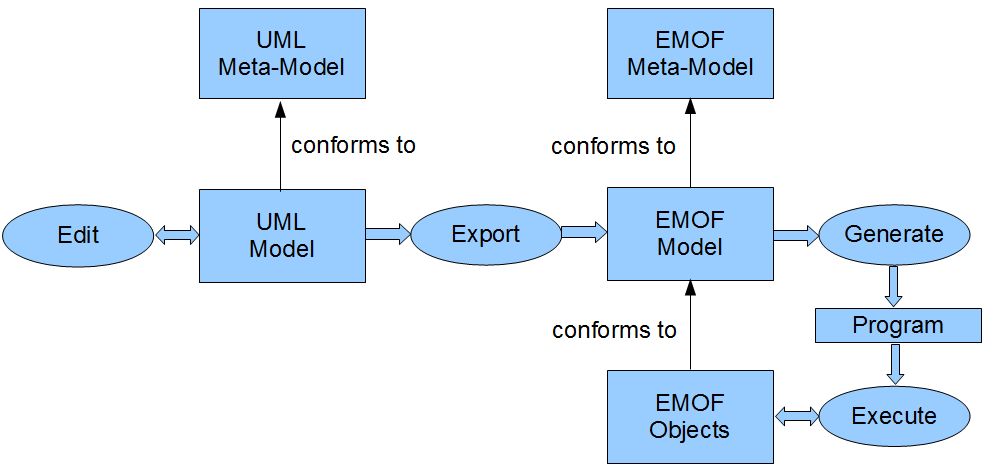
\includegraphics[width=5.75in]{BasicScenario.png}
  \end{center}
  \caption{Basic Scenario for executable usage of UML.}
  \label{fig:BasicScenario}
\end{figure}

The UML meta-model defines a rich suite of capabilities suitable for meta-modeling. The export to the EMOF meta-model reduces the capabilities to those necessary to support effective use of models at run-time.

When we add OCL capabilities, and ignore model execution, in order to simplify the diagram, we get the scenario shown in Figure~\ref{fig:BasicOCLScenario} for developing a UML model that includes constraints.

\begin{figure}
  \begin{center}
    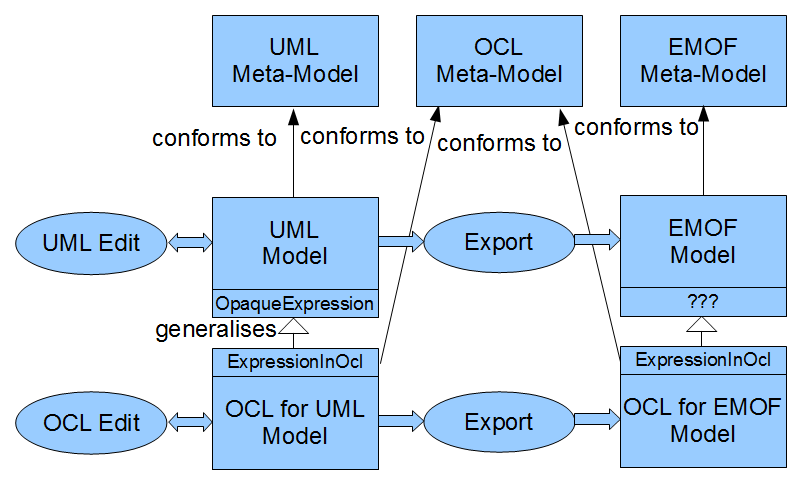
\includegraphics[width=4.5in]{BasicOCLScenario.png}
  \end{center}
  \caption{Basic OCL Integration Scenario.}
  \label{fig:BasicOCLScenario}
\end{figure}

The OCL integration with UML is quite tidy with OCL providing an ExpressionInOcl class that extends UML's OpaqueExpression class. The very different characteristics of graphical UML and textual OCL typically require distinct editors.

The corresponding EMOF integration is troublesome because EMOF has discarded too many UML concepts that OCL requires. EMOF has no ValueSpecification or Constraint to contain the ValueSpecification from which OpaqueExpression and ExpressionInOcl derive. More generally EMOF has no Association or Classifier classes and so the OCL for UML and OCL for EMOF models have significant differences that make it doubtful that they both conform to the one OCL Meta-Model.

The limitations of EMOF are accommodated in the specification by Clause 13 that provides an open list of OCL functionality that is not applicable to EMOF. Some exclusions such as Messages represent a plausible sub-language; others concerning Associations and missing classes are a mis-alignment. The failure to support Complete OCL for EMOF seems untenable.

Nonetheless, if we ignore these EMOF issues for now, and just treat UML/EMOF and OCL in combination, and then consider evaluation of constraints defined in the meta-model upon a model, we get Figure~\ref{fig:M2Evaluation}.

\begin{figure}
  \begin{center}
    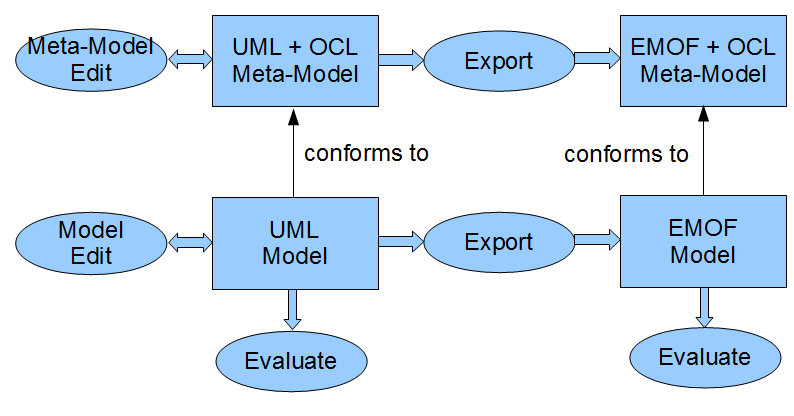
\includegraphics[width=4.5in]{M2Evaluation.png}
  \end{center}
  \caption{M1 Evaluation for UML or EMOF.}
  \label{fig:M2Evaluation}
\end{figure}

When we consider the desirable characteristics of the different ways that models are used we find:
\begin{itemize}
\item Definition of models requires the richness of UML
\item Execution of models benefits from the slimmed down efficient characteristics of EMOF 
\item Definition of OCL constraints requires much of the richness of UML
\item Evaluation of OCL constraints benefits from a slimmed down efficient representation
\end{itemize}

The last two OCL considerations pull in opposite directions; a rich OCL + UML environment for development and an efficient environment for evaluation. Neither is compatible with UML or EMOF characteristics. UML is too rich for efficient execution and EMOF is too limited for adequate expression capability.

The current OCL specification with its statement that OCL can be used with both UML and EMOF is unhelpful and unrealistic. The deficiencies for EMOF behavior are too great. Tool implementers are forced into pragmatic solutions to support more than one of EMOF and UML. 

We will therefore propose, in Section \ref{PivotMetaModel},  a combined UML and OCL Pivot Meta-Model that exhibits the more efficient characteristics of EMOF while retaining the relevant richness of UML.

\section{Problems}\label{Problems}

\subsection{Complete OCL Problems}\label{CompleteOCL}

A Complete OCL document can complement a model and add features to it so that they can be used as if they were part of the complemented model. Additional features may be added to library types as well, so definition of an \verb|OclAny::isPersistent()| operation may add an ability to evaluate constraints concerning the persistent storage associated with any model element.

The additional Abstract Syntax for Complete OCL comprises just the ExpressionInOcl class. Unfortunately problems arise when we try to realize the first paragraph of Clause 12.5 which states:

``A definition constraint is a constraint that is linked to a Classifier. It may only consist of one or more LetExps. The
variable or function defined by the Let expression can be used in an identical way as an attribute or operation of the
Classifier. Their visibility is equal to that of a public attribute or operation. The purpose of a definition constraint is to
define reusable sub-expressions for use in other OCL expressions.''

[We will ignore the reference to LetExps that refers to an obsolete OCL 1.x concrete syntax and so makes the paragraph difficult to interpret for OCL 2.x.]

The subsequent description and figure show that the definition is realized by an ExpressionInOcl that is indirectly owned by the context classifier via a Constraint. The figure is redrawn as Figure \ref{fig:Definition} which corrects trivial UML misalignments. 

\begin{figure}
  \begin{center}
    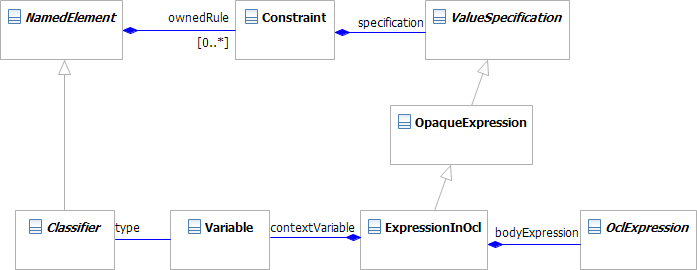
\includegraphics[width=5.75in]{Definition.png}
  \end{center}
  \caption{Specified relationship of a Definition to a Classifier.}
  \label{fig:Definition}
\end{figure}

The intent of ``an identical way as an attribute or operation'' is clear. A defined property or operation must be usable in an OCL expression, and so must be usable in both concrete and abstract syntax as if the definition formed part of the complemented model.

Utility in the concrete syntax requires that the Environment lookup is able to locate the definition by hierarchical name. The specification of Environment lookup in Clause 9 can resolve Property and Operation model elements. Unfortunately the Inherited Attribute rules are missing from Clause 12 so it is unclear how a Property or Operation is resolvable from an object structure that does not include such a feature. It is also unclear how a definition is able to export a name into the Environment in the reverse direction to that for inherited attributes.

Utility in the abstract syntax means that a PropertyCallExp::referredProperty or an OperationCallExp::referredOperation is able to refer to the definition. This requires that the definition is either a Property or an Operation. None of the Constraint, ExpressionInOcl or OclExpression classes shown in Figure \ref{fig:Definition} satisfy this requirement.

These considerations all indicate that the abstract syntax must be revised so that a definition is realized by a Property or Operation as shown in Figure \ref{fig:PropertyDefinition}. With definition realized by features in models, the problem of installing the definition for lookup in the Environment is resolved; the definitions are installed in the same way as any other feature. The lookup results are features and so can be the target of references from the existing expression abstract syntax.

\begin{figure}
  \begin{center}
    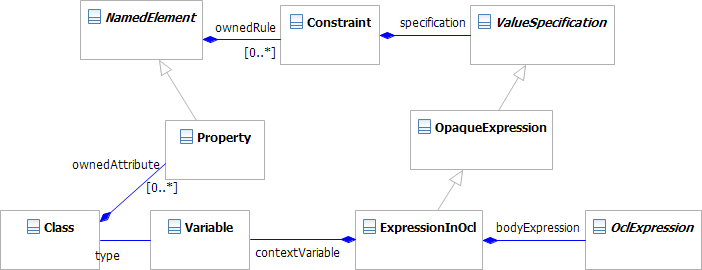
\includegraphics[width=5.75in]{PropertyDefinition.png}
  \end{center}
  \caption{Property relationship of a Definition to a Classifier.}
  \label{fig:PropertyDefinition}
\end{figure}

This creates a minor problem for UML alignment. A Property is added to a Class rather than a Constraint to a Classifier, which is a bit clumsy since the realization of ownedAttribute differs between PrimitiveType and Class.

We have one more major problem to solve. What is the relationship between the Class which Complete OCL complements with a definition and the Class for which the definition is an ownedAttribute or ownedOperation? We will examine this problem shown in Figure \ref{fig:MultipleModels} from a variety of perspectives. (The figure is mis-drawn using class rather than attribute notation to highlight the distinct elements involved.)

\begin{figure}
  \begin{center}
    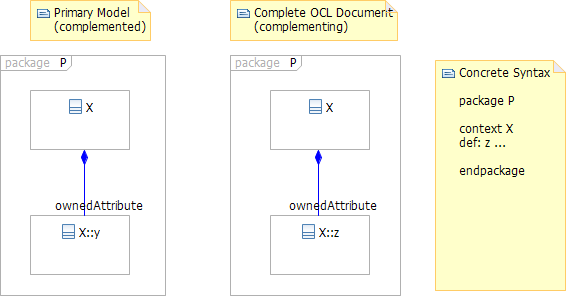
\includegraphics[width=3.5in]{MultipleModels.png}
  \end{center}
  \caption{The Multiple Models problem for Complete OCL.}
  \label{fig:MultipleModels}
\end{figure}

\subsubsection{Merged or Multiple models}

The simplest solution is that the two Package P's and the two Class X's are combined to form merged Package P and  Class X objects. However this means that the Package P and the Class X in the UML model are modified by usage of Complete OCL.

The alternative is to maintain some form of composite model in which multiple contributory models are treated as a coherent composite whole.

\subsubsection{Model Maintenance}

The merged model is a normal model and so should be amenable to support by a UML modeling environment. However since the model is modified, it may be necessary to create a distinct model for each usage, since each usage may have a different combination of Complete OCL documents. The Complete OCL complements for one usage must not infect another usage.

The composite model comprises multiple unmodified normal models, so these contributions can be shared between usages. However special functionality is required to allow the composite to behave coherently. This functionality will not be directly available from a UML modeling environment.

\subsubsection{Implicit Access}

Implicit access occurs through navigation of a property or invocation of an operation in an OCL expression.

For the merged model this presents no new problems since the merged model is internally coherent.

For the composite model the OCL tooling is able to intercept the access and so direct the implicit access to the appropriate contributory model.

\subsubsection{Explicit Access}

Explicit access occurs when reflection is used to access the properties. Since reflection is not consistently specified ion OCL 2.3, there is discretion as to how this is specified in the future.

In Figure \ref{fig:MultipleModels}, should the reflective access to X::ownedAttribute return both X::y and X::z hiding the distinct origins of the two features, or should there be a mechanism to obtain distinct ownedAttributes from each?

The merged model can only present the coherent view. Additional features are needed to enable helper operations to provide partial returns.

The composite model naturally supports the disjoint view and helper operations can provide a merged view. Reflection can allow expression access to see disjoint or coherent views.

\subsubsection{URIs}

When a reference to a complementing definition is persisted via XMI, a URI must be established for the definition so that the complementing definition can be reconstructed when the XMI is loaded.

The merged model will naturally provide URIs appropriate to the merged context, which solves the problem of providing a URI, but the merged context is unhelpful for reload, since the distinct identity of the Complete OCL document is obscured, unless some special form of URI is used to capture the distinct origin.

The composite model preserves the distinct model identities and so will naturally provide URIs that correspond to the relevant document.

\subsubsection{Summary}

Neither approach is entirely satisfactory. The merged model has significant problems with sharing, URIs and full reflection. The composite model has fewer problems requires additional non-UML tooling to represent the composite. In Section \ref{PivotMetaModel} we propose a solution that builds upon the composite model.

\subsection{EMOF Problems}

\subsubsection{How does a Complete OCL definition apply to an EMOF model?}

OCL is specified to apply to both UML and EMOF models, except that a reduced functionality applies where EMOF has no support for required concepts.

In the case of additional features, full EMOF functionality is specified despite EMOF's lack of support for adding features to data types. Clause 13.2 bullet 6 suggests a convention is introduced whereby an accompanying class instance is provided for such types. This recommendation ignores the absence of a solution for Constraint and OpaqueExpression in EMOF that makes OCL integration impossible without an extended OCL Abstract Syntax.

This is an uncomfortable workaround for the lack of UML alignment. It causes difficulties for tools since features are no longer defined in just one place, so the default functionality of a generic modeling framework such as Ecore must be adjusted so that all functionality that can see the meta-model features also see the accompanying class instance features. Achieving this consistently for reflective functionality is perhaps impossible since any attempt to access the container of the accompanying class instance will discover that is  an accompaniment.

\subsection{Other Problems}

\subsubsection{Iterator Operation}

The iterate and iterator operations have no UML counterpart and so cannot be represented by a UML meta-model. As a result, all support for iterators requires built-in functionality, and indeed prior to OCL 2.3, the specification could be interpreted to require all names of iterators to be hard-wired into the OCL grammar. OCL 2.3 clarified the status of names so that any name can be used as an iterate or iterator operation.

In our Companion paper\cite{OCL-stdlib} we show how introduction of an Iteration class extending the Operation class is sufficient to allow the OCL Standard Library to be modeled.

\subsubsection{OclAny conformance}

OCL uses the conformsTo relationship between types to determine substitutability. This relationship is almost identical to UML generalization; the main difference being the definition that all UML classes conform to OclAny.

Direct realization of the above leads to some practical difficulties. Firstly the lookup of matching features must use one algorithm to traverse the generalization hierarchy, and another to extend on to OclAny. This irregularity becomes more of a concern when considering a UML operation such as \verb|Classifier::conformsTo()| which traverses the generalization hierarchy and so requires that OclAny is part of the generalization hierarchy.

\subsubsection{Reflection}

The \verb|OclAny::oclType()| operation was added to the OCL Standard Library when it was realized that the MOF \verb|Element::getMetaClass()| operation was not accessible for UML meta-models, which do not merge MOF.

Since OCL mandates that all types conform to OclAny, use of \verb|OclAny::oclType()| requires that all types at all meta-levels must conform to OclAny.   

\section{Solutions}\label{Solutions}

\subsection{OCL Pivot Meta-Model}\label{PivotMetaModel}

We can accommodate the conflicting UML-alignment requirements in a variety of ways.

We could eliminate all non-UML facilities from OCL, but OCL without Iterations would not be of much utility, so this is untenable.

We could eliminate the statement that OCL is aligned with UML. This is pretty much unthinkable given UML's dependence on OCL.

We could revise UML so that it supports the facilities that OCL requires. This is possible in principle, but hardly desirable since it may incur political difficulties and further practical difficulties in mutual alignment.

In order to make OCL useful for EMOF meta-models we could add the missing parts of UML such as Associations and OpaqueExpressions to OCL. This can solve the EMOF problem but creates inconsistencies whereby OCL provides additional classes solely for use in a simple context.

In the following sections we will therefore pursue an alternative approach whereby we re-use the constructive nature of the UML specification to select those packages that are relevant and then merge these with additional OCL packages to create a new UML-derived OCL Pivot Meta-Model.

With the OCL Pivot Meta-Model UML-derived, large parts will automatically be UML-aligned, but we are able to adjust any UML well-formedness rules that are not applicable to OCL since the UML and OCL meta-models are distinct.

As a pivot model, the OCL Pivot Meta-Model is neutral and so independent of UML or EMOF and so can be used in conjunction with  a variety of alternate meta-models.

The OCL Pivot Meta-Model is a complete and follows the trend of ensuring that major meta-models are self describing. In UML 2.4, a UML::Class has a UML::Class as its meta-class. For the proposed UML-derived OCL Pivot Meta-Model, an OCL::Class has an OCL::Class as its meta-class.  


\subsubsection{Meta-Meta-Model Merge}

The OCL Pivot Model is a Meta-Meta-Model with respect to user models. The OCL Pivot model is derived by the package merge  shown in Figure~\ref{fig:UMLMMtoOCLMM}.

\begin{figure}
  \begin{center}
    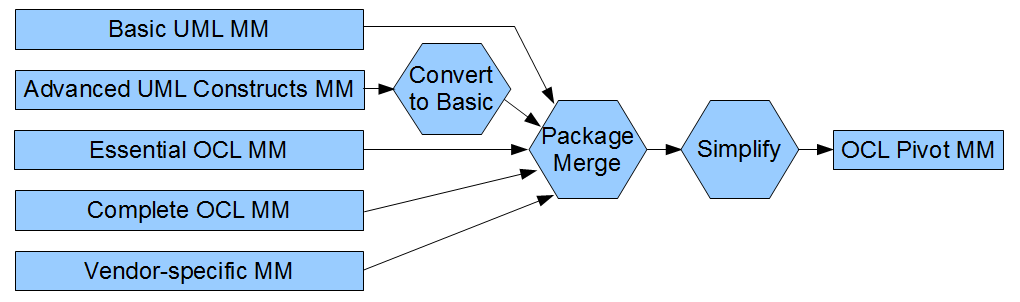
\includegraphics[width=5.75in]{UMLMMtoOCLMM.png}
  \end{center}
  \caption{Meta-Model merge to produce the OCL Pivot Meta-Model.}
  \label{fig:UMLMMtoOCLMM}
\end{figure}

The contributions to the merge are:

\subparagraph{Basic UML}

The UML InfrastructureLibrary::Core::Basic package defines the Essential MOF. It provides efficient but inflexible representations of each class. For instance, subset properties are eliminated so that an Operation is found in Class::ownedOperation, but not in Class::feature or Namespace::member or Namespace::ownedMember or Element::ownedElement.

\subparagraph{Additional UML}

OCL Constraint integration requires the InfrastructureLibrary::Core::Abstractions::Constraints package.

Full type support requires the InfrastructureLibrary::AuxiliaryConstructs::Templates package.

OCL Message support requires the UML::Actions::BasicActions package to define CallOperationAction and CallOperationAction. and the UML::CommonBehaviors::Communications package to define Signal.

OCL State support requires the UML::StateMachines::BehaviorStateMachines package to define State.

Unfortunately these packages were not intended to be merged into Basic, so they do not provide the same efficient representation. The Eclipse OCL prototype works around this problem by manual creation of `Basic' equivalents.

It is possible that the UML simplification process\cite{UML-simple} may eliminate the Basic package as a primary artifact, and exploit a QVT Operational transformation to derive it. It may be appropriate to enhance this transformation to also derive basic variants of other relevant packages.

\subparagraph{Essential OCL}

These are the packages defined by Clause 8 of the current OCL specification, with minor enhancements to align with UML. 

\subparagraph{Complete OCL}

This is the single class package defined by Clause 12 of the current OCL specification, with some revision to align with UML. 

\subparagraph{Vendor-specific}

The package merge is not constrained to the requirements of the OCL specification. Tool vendors may merge further packages to support visitor protocols, useful operations or transient caches.

\subparagraph{Simplify}

In completion of the package merge the meta-model can be simplified to eliminate redundant classes such as Type, remove redundant generalizations and convert the remainder to conformance.

\subsubsection{Meta-Model Load}

Before any evaluation on a user model can occur, its meta-model must be loaded. This currently presents challenges since users may use a variety of UML, CMOF, EMOF and Ecore dialects not all of which are supported by all tools. With a neutral Pivot Model the diverse sources are accommodated by a variety of compilation or loading activities as shown in Figure~\ref{fig:Load}.

\begin{figure}
  \begin{center}
    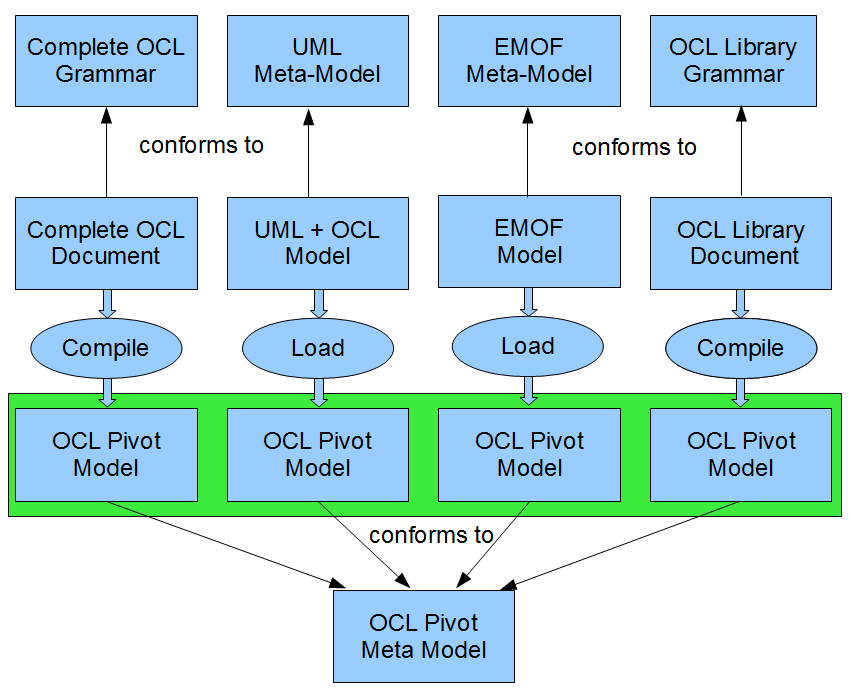
\includegraphics[width=4.75in]{Load.png}
  \end{center}
  \caption{Composite Pivot Model derived from disparate sources.}
  \label{fig:Load}
\end{figure}

Introduction of the OCL Pivot Meta-Model requires the user meta-model to be converted to, or at least interpreted in, a normalized form. In this respect the proposed OCL Pivot is similar to that advocated by Wilke\cite{Variability} as a Meta-Model Variation Point to support meta-model representation diversity.

The new meta-model load phase enables the following problems to be resolved:

\begin{itemize}
\item Diverse meta-model dialects can be intermixed
\item Complete OCL documents can be represented as OCL Pivot Models
\item OCL Standard Libraries can be represented as OCL Pivot Models
\item UML generalization can be re-interpreted as OCL conformance
\item OclAny can be inserted into the conformance hierarchy
\end{itemize}

With all OCL concepts consistently modeled, the OCL Pivot Meta-Model can be used to provide the URIs needed to solve the problem of XMI interchange.

With a normalized meta-model representation, limitations in OCL support such as navigating non-navigable associations are caused by limitations in the meta-model loader rather than in OCL. OCL is fully specified for such associations, but they are useable for EMOF only when the \verb|org.omg.emof.oppositeRoleName| tag introduced in MOF 2.4\cite{MOF-2.4} is exploited by both meta-model producer and consumer.

\subsection{Primitive Types and Values}\label{Values}

The representation of a value in OCL appears to be very similar to conventional languages, but is actually very different. We will therefore examine the issue carefully.

\subsubsection{Primitive Values}

UML provides a PrimitiveTypes package that defines the primitives, such as Integer or String, as a domain of values without specifying any representation or behavior. This vagueness for primitives is important to allow a UML model to specify the required behavior of a wide variety of alternate implementations without imposing a particular representation. Each primitive is an instance of the PrimitiveType metaclass.

\begin{figure}
  \begin{center}
    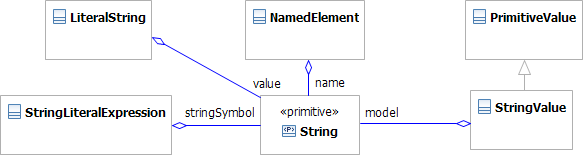
\includegraphics[width=5.75in]{String.png}
  \end{center}
  \caption{The String primitive attributes and their `containers'.}
  \label{fig:String}
\end{figure}

A primitive, as shown in Figure~\ref{fig:String}, can only exist within a suitable `container', such as the NamedElement::name Property that binds a String to perform the role of naming its NamedElement.  For a more general purpose role such as a string value, UML defines LiteralString which subtypes the polymorphic ValueSpecification. Similarly OCL defines a string role in an expression using StringLiteralExpression which subtypes the polymorphic OclExpression. The progression NamedElement::name, LiteralString::value to StringLiteralExpression::stringSymbol provides steadily richer roles, but does not specify any representation or behavior for use in that role.

 It is the OCL Standard Library that specifies primitive and non-primitive behavior, and it is the OCL Values package that specifies an OCL representation for which that behavior applies. 

In order to evaluate an operation such as String::toUpperCase() on a string, the string must be contained in a context that supports that operation evaluation. This is a StringValue in OCL. This is confusing to anyone familiar with almost any Object Oriented Language, since String is conventionally a class that provides a rich suite of behaviors. In UML and OCL, a primitive String has no associated representation or behavior. It  is only as the model of a StringValue that behavior defined by the OCL Standard Library is usable.

This confusion is compounded by practical OCL implementations that may reuse the String type of their implementation language to realize the StringValue representation and behavior for OCL. This reuse can work very effectively for basic functionality, but is troublesome for precise functionality, since it is unlikely that a practical OO Language will have exactly the same semantics as OCL. For instance, consider the irregularity whereby the UnlimitedNatural for an unlimited value (plus-infinity)  is invalid once the UnlimitedNatural is interpreted as either of Integer or Real to which UnlimitedNatural conforms.

It is also tempting to use the Collection capabilities of an implementation language to directly implement the OCL CollectionValue representations and behaviors. However considerable care may be required to ensure that for instance \verb|OrderedSet{Set{4.0}}->including{Set{4}}->size()| is 1 rather than 2, since the encapsulated equality of 4.0 and 4 may not be respected by the language semantics.

Maintaining the separation between behavioral representation and implementation representation for primitive values as specified by Clause 10.2 has considerable advantages; the behavioral Value layer delegates to implementation types, but can impose OCL semantics consistently prior to delegation. The Value layer may therefore provide a behavioral inheritance hierarchy that matches the OCL primitive type hierarchy and so it does not matter whether the implementation language has that hierarchy or not.

Unfortunately Clause 10.2 is very deficient in supporting this view. There is a StringValue class that conforms to a PrimitiveValue class, but no BooleanValue, NumericValue or IntegerValue classes. Clause 10.2  does not define any features for the PrimitiveValue classes, so they appear to fail to fulfill their role of containing a primitive value. However in Clause 10.4, Figure 10.14 provides a consistent model property for primitive Values, although unfortunately again Figure 10.14 as a whole is very deficient through a variety of meta-level confusions. Significant revision of Clause 10 is required to support the actual OCL (and UML) primitives.

\subsubsection{Object Values}

The benefits of the Value hierarchy imposing consistent semantics independent of the underlying implementation for primitive and collection values is equally applicable to object values.

OCL 2.3 specifies an ObjectValue class that maintains object history using a sequence of LocalSnapshot instances. The  ObjectValue::getCurrentValueOf(String) method determines the prevailing value of an object property. This specification. right at the start of Clause 10, far exceeds what is necessary for practical tooling and probably explains why practical tools have ignored the entire clause and realized values  much more simply by direct use of implementation language types and modeling environment objects. And equally, since the clause is irrelevant to actual tools, the specification maintainers have failed to understand the clause and consequently Clause 10 has far more errors than any other part of the specification.

Object history is useful to define the foundation for the semantics of pre- and post-conditions and of message histories, since the relationship between two system states must be specified. However, a simple cache of @pre expressions is all that is necessary to support pre and post conditions, and a selective trace of object activity can support OclMessage. No history at all is required by implementations that don't offer the @pre and message compliance points.

However discarding Clause 10 completely and using model objects directly loses the polymorphism and couples the OCL tooling to a particular model object representation. Wilke\cite{Variability} recognized this limitation as the Model Instance Variation Point and introduced Model Instance adapters to accommodate the different object representations of Java, Ecore, XML or Relational Data. It is ironic that this is what the OCL Specification already requires through ObjectValue polymorphism. While maintenance of history may be an excessive implementation burden, using a derived XMLObjectValue to mediate between the neutral OCL evaluation engine and the XML specific representation is eminently sensible and necessary to provide an ObjectValue as the object representation.

\begin{figure}
  \begin{center}
    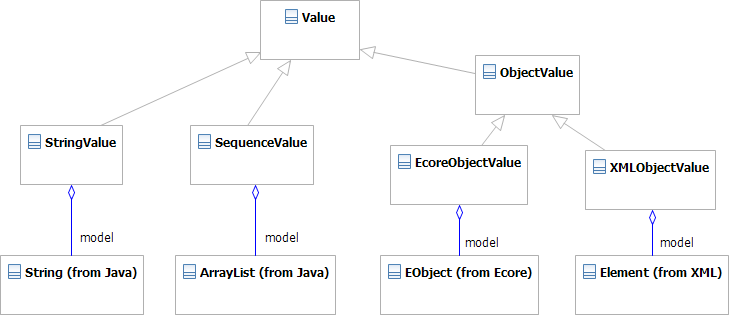
\includegraphics[width=5.75in]{Value.png}
  \end{center}
  \caption{Practical simplified OCL Value hierarchy for a Java tool.}
  \label{fig:Value}
\end{figure}

Adopting this approach, a Java-based tool, might choose to delegate StringValue and SequenceValue directly to Java's String and ArrayList classes as shown in Figure~\ref{fig:Value}, while introducing an adapting layer of EcoreObjectValue or XMLObjectValue for specific Object representations.

The OCL specification already requires that all values to be maintained by derived Value class instances within an evaluation. Once this aspect of the specification is implementable and realized by tools, interchange within sub-tools may be easier. 

\subsection{Details}

In previous sections we have described significant changes that are required. In this section we identify a variety of comparatively small misalignments between UML and OCL and consider whether and how they might be resolved.

\subsubsection{Primitive Types}

UML 2.4 has moved the Primitive Types to a separate package to facilitate reuse and defined the previously missing Real type that OCL needed to use. OCL can therefore reuse this UML package.

\subsubsection{Types}

UML has distinct Type, Classifier and Classes, but OCL allows features to be added to any type eliminating the major difference between the three UML classes. All three UML classes can therefore be merged into one. The main challenge is to decide which name to use in the merged OCL Pivot Meta-Model. UML has Package::ownedTypes and Class::superClasses and we want to avoid UML users needing to learn a new or inconsistent vocabulary for the OCL Pivot Meta-Model, so these names should persist. Type and Classifier all become Class reflecting the availability of Class functionality for all types.

Of course with all types uniform, the need for companion classes to support Complete OCL operations on data types is eliminated.

\subsubsection{Iteration}

With the OCL Pivot meta-model derived from UML by package merge, it is not necessary to modify UML in order to introduce an Iteration class. OCL can just define an Iterations package to contribute to the overall merge.

If it is felt appropriate for UML, the Iterations package can be promoted to UML, but this would run very counter to the drive to simplify UML, so the extra merge solely for OCL seems a more satisfactory solution. 

\subsubsection{ExpressionInOcl}

ExpressionInOcl is shown as deriving from OpaqueExpression in the first figure of Clause 12; this is aligned with UML. Unfortunately the remaining figures and editorial text all use derivation from Expression which is inappropriate but easily corrected.

\subsubsection{Definition Constraints}

The Abstract Syntax for definitions installs definitions as constraints on their containing type, although the installed definitions exhibit behavior indistinguishable from features. The proposed OCL Pivot Meta-Model supports realization of definitions as features in a parallel model.

\subsubsection{Qualified Associations}

The Concrete and Abstract syntax for qualified associations has never been quite right and has become less so as partial evolution with UML has been applied.

There is no abstract syntax for \verb|self.associationEndName[qualifiers]| since PropertyCallExp does not support qualifiers.

There is no abstract syntax for \verb|self.associationClassName[qualifiers]|, since AssociationClassCallExp does not support qualifiers.

There is no abstract or concrete syntax for the doubly qualified navigation that may arise with a recursive ternary association class, since AssociationClassCallExpCS does not support qualifiers.

Alignment with UML therefore requires a correct initial specification rather than maintenance. 

\subsubsection{AssociationEnd}

All residual references to AssociationEnd must be revised to use Property.

\subsubsection{Expression and OclExpression}

UML provides for a homogeneous Expression tree in which nodes have a String name and an arbitrary number of operands.

OCL provides for a heterogeneous OclExpression tree in which nodes have node-specific content such as OperationCallExp::referredOperation.

Both forms of expression integrate with UML classes as the derived ValueSpecification of a Constraint.

Are two distinct trees appropriate? The OCL Abstract Syntax could be revised to extend Expression, but this would involve significant incompatibilities without any obvious benefit. OCL tools benefit from the richer Abstract Syntax, so stronger UML alignment of OclExpression does not seem appropriate.

\subsubsection{LiteralSpecifications and LiteralExpressions}

UML defines a LiteralString and OCL defines a StringLiteralExpression. These classes have very similar inheritance from TypedElement and could be merged, perhaps introducing a derived property to permit use of both stringSymbol and value property names, perhaps migrating OCL to eliminate the unnecessary repetition in unlimitedNaturalSymbol.

If merged, LiteralExpression would need to extend LiteralSpecification, allowing use of OCL literals more directly in UML Constraints without a wrapping ExpressionInOcl. If OclExpression similarly extended ValueSpecification, then constant expressions, requiring no self, could also be used directly.

This is relatively minor tweaking, for which there is no obvious demand. However since it could easily accommodated by the UML to OCL merge, it is perhaps worth doing. But it doesn't work, the hybrid OCL::LiteralString and OCL::StringLiteralExpression would extend OCL::ValueSpecification rather than UML::ValueSpecification, so a derived UML::OpaqueExpression wrapper would still be needed to permit use of OCL within UML. Therefore the UML Literals package can be mapped to LiteralExpressions so that the OCL tooling for pivot models does not need to handle two alternative forms of literal. 

\subsection{Practice}

The way the OCL Pivot Meta-Models work in practice is shown in Figure~\ref{fig:M0Evaluation} for evaluation at M0 and Figure~\ref{fig:M1Evaluation} for evaluation at M1. In each case the objects on which we evaluate are wrapped as OCL Values which conforms to an OCL Pivot Model defined by the user object's model. The OCL Pivot Model conforms to the OCL Pivot Meta-Model. The OCL evaluation operates entirely in the OCL domain; the differences between UML or EMOF (or Ecore) are relegated to the load activity that creates the OCL Pivot Model.

\begin{figure}
  \begin{center}
    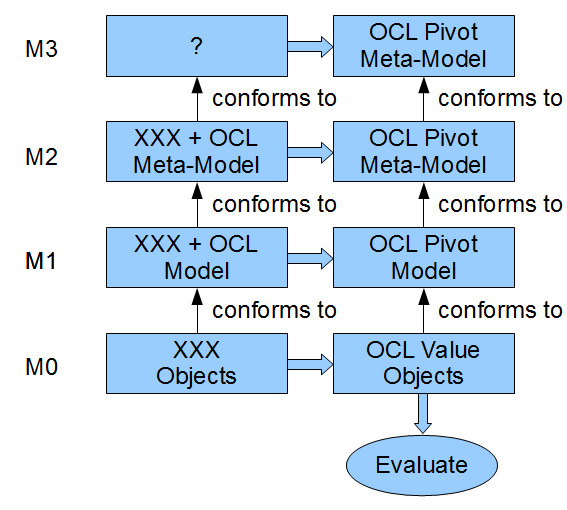
\includegraphics[width=2.75in]{M0Evaluation.png}
    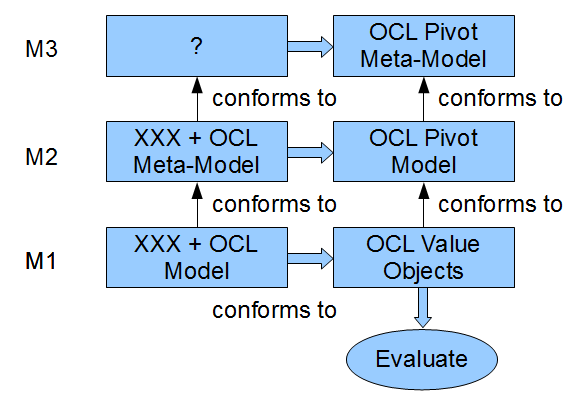
\includegraphics[width=2.75in]{M1Evaluation.png}
  \end{center}
  \caption{M0 Evaluation.}
  \label{fig:M0Evaluation}
  \caption{M1 Evaluation.}
  \label{fig:M1Evaluation}
\end{figure}

\section{Conclusions}

We have identified major problems in the OCL specification in regard to URIs for XMI Interchange and a coherent Abstract Syntax for Complete OCL.

A UML-derived OCL Pivot Meta-Model has been introduced to solve these problems and we have shown how this solves other problems such as UML-alignment, meta-model diversity, reflection, conformance modeling and OCL Standard Library modeling as well. The OCL Pivot Meta-Model decouples an OCL implementation from UML and EMOF and so facilitates meta-model diversity.

Examination of the OCL Values Package has revealed that it requires a similarly decoupling from model representations. This requirement should be clearly expressed in the specification so that value interchange between OCL tools is possible. 

\nocite{*}
\bibliographystyle{eceasst}
\bibliography{AligningOCLandUML}

\end{document}

